\section{Colisiones en el Plasma: Secciones eficaces y frecuencias de colisi\'on. Introducci\'on cualitativa desde una perpectiva en 1D}

  En est\'a secci\'on introduciremos de modo cualitativo los distintos conceptos fundamentales en el \'ambito de colisiones, si bien est\'as en algunos casos no son las expresiones generales usadas para casos m\'as amplios y modelos m\'as complejos, introduce de manera simple los conceptos bases en los que se fundamentan los modelos cin\'eticos. 

  Las colisiones m\'as simples que pueden presentarse en un plasma son aquellas entre electrones con \'atomos neutros, estas pueden ser el\'asticas, lo que significa que ambas especies mantienen su identidad y en modelos simples los electrones simplemente rebotan de los neutros, se asume que el cambio de momento de los \'ultimos es negligible. Luego est\'an las colisiones inel\'asticas, en este caso se dan procesos de ionizaci\'on, radiaci\'on, recombinaci\'on. Entre especies con carga neta en el plasma tambi\'en se pueden encontrar las llamadas colisiones de Coulomb, que como su nombre lo indica se dan por interacciones de Coulomb entre las part\'iculas del plasma. 

  A groso modo, estos eventos mencionados pueden estudiarse desde la estad\'istica usando el concepto de probabilidad y secciones eficaces. Por ejemplo, para una colisi\'on el\'astica o inel\'astica se puede definir la secci\'on eficaz $\sigma$ que es el \'area transversal, si modelamos las part\'iculas como esferas, que tendr\'ia la part\'icula si al colisionar un electr\'on con el neutro, este se reflejara en un \'angulo de $90^\circ$ o si el \'atomo se ionizara con todos los electrones que lo colisionan.

    Sea $n_0$ la densidad de neutros que hay en un plasma, se define el camino libre medio $\lambda_{mfp}$ como el recorrido promedio que tendr\'a el electr\'on antes de tener una probabilidad de colisionar con otro neutro \cite{goldston1995}. 

    Introduciremos un simple ejemplo en el caso 1D de forma ilustrativa. Imaginese un loza de grueso $dx$ con neutros, ve\'ase la figura abajo. La cantidad de estos por unidad de \'area es de $n_0dx$ y el \'area que ocupan en la loza es de $n_0 \sigma dx$. 

    \begin{figure}[hbt!]
 		\label{fig:slabdx}
 		\centering
 		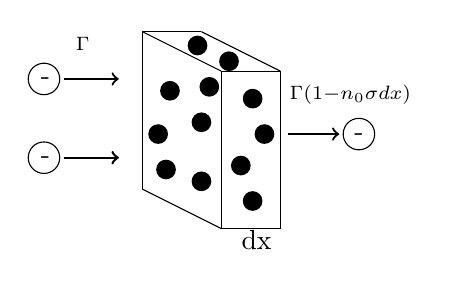
\begin{tikzpicture}
 			\draw (0,0) -- (0,2);
 			\draw (1,-0.5) rectangle (1.75,1.5);
 			\draw (0,0) -- (1,-0.5);
 			\draw (0,2) -- (1,1.5);
 			\draw (0,2) -- (0.75,2);
 			\draw (0.75,2) -- (1.75,1.5);
 			\fill (1.4,-0.15) circle (0.125);
 			\fill (1.4,1.15) circle (0.125);
 			\fill (1.25,0.3) circle (0.125);
 			\fill (1.55,0.7) circle (0.125);
 			\fill (1.1, 1.625) circle (0.125);
 			\fill (0.7, 1.825) circle (0.125);
 			\fill (0.3,0.25) circle (0.125);
 			\fill (0.2,0.7) circle (0.125);
 			\fill (0.35,1.25) circle (0.125);
 			\fill (0.75,0.1) circle (0.125);
 			\fill (0.75,0.85) circle (0.125);
 			\fill (0.85,1.3) circle (0.125);
 			\draw (-1.25,1.4) circle (0.2);
 			\node at (-1.23,1.4) {-};
 			\draw (-1.25,0.4) circle (0.2);
      \draw[->, thick] (-1.0, 0.4) -- (-0.3,0.4);
      \draw[->, thick] (-1.0, 1.4) -- (-0.3,1.4);
      \node at (-1.23,0.4) {-};
 			\draw[->, thick] (-1.0, 0.4) -- (-0.3,0.4);
  		\node at (1.45,-0.65) {dx};
  		\node at (-0.75,1.85) {$_\Gamma$};
  		\draw[->, thick] (1.85, 0.7) -- (2.5,0.7);
  		\draw (2.75,0.7) circle (0.2);
  		\node at (2.75, 0.7) {-};
  		\node at (2.65, 1.2) {$_{\Gamma(1 - n_0\sigma dx)}$};
 		\end{tikzpicture}
 		\caption{Flujo de electrones $\Gamma$ incidente sobre una loza de grosor $dx$ que contiene una densidad de neutros $n_0$.}
 	\end{figure}

    Hacia la loza hay un flujo de electrones perpendicular al \'area transversal de la loza, este flujo incidente los llamaremos $\Gamma(x)$, ya que consideramos los neutro como esferas r\'igidas de secci\'on efectiva, si un electr\'on colisiona con un neutro habr\'a ionizaci\'on por lo qque el flujo de electrones no es el mismo que sale, el flujo de electrones que no colisiona con los neutros est\'a dado por $\Gamma + d\Gamma = \Gamma(1 - n_0\sigma dx)$ De esto se obtiene que, el cambio de $\Gamma$ con la distancia $x$ est\'a dada por 

    \begin{eqnarray}
      \frac{d\Gamma}{dx} &=& -n_0\sigma \nonumber\\
      \implies \Gamma(x) &=& \Gamma_0\exp{(-n_0\sigma x)} \nonumber
    \end{eqnarray}
  
    N\'otese que $n_0\sigma$ tiene unidades de $m^{-1}$, se define $\lambda_{mfp} = (n_0\sigma)^{-1}$ como el camino libre, trayecto recorrido a partir del cual existe una probabilidad razonable de colision con un neutro \cite{goldston1995}. Para los casos de inter\'es existe un $\lambda_{mfp}$ cuantitativamente distinto al de este caso, pero la definici\'on cualitativa es la misma.

  Para electrones con velocidad $v$ el tiempo medio entre colisiones es

  \begin{equation}\label{eq:tmc}
    \tau = \lambda_{mfp}/v
  \end{equation}

  Al inverso de esta cantidad se le denomina ''frecuencia de colisi\'on'' y se define en t\'erminos de una funci\'on de distribuci\'on como
  
  \begin{equation}\label{eq:freq}
    \nu = \left<\tau^{-1}\right> = n_0\left<\sigma v\right> = \frac{n_0}{n_e}\int d^3 f_e(v)\sigma(v)v
  \end{equation}

  Para cada tipo colisi\'on se puede asignar una frecuencia de colisi\'on de la cual se puede obtener la tasa en la que cada evento da paso a perdida o adici\'on de part\'iculas de una u otra especie en el plasma, al multiplicar estas frecuencias por la densidad de las part\'iculas se obtiene un t\'ermino $N_{evento}$ que es la tasa de emisi\'on o fuente, este es el n\'umero de eventos (colisiones que provocan ionizaci\'on, radiaci\'on, colisiones de Coulomb, recombianciones, etc) que se dan por segundo en un determinado volumen \cite{lechte2002}.

  \begin{equation}\label{eq:events}
    N_{evento}(T_\alpha) = n_\alpha n_\beta\left<\sigma v\right>_{evento}(T_\alpha) 
  \end{equation}

  Las expresiones de las Ecs. \eqref{eq:tmc}, \eqref{eq:freq} y \eqref{eq:events} s\'i son definiciones cuantitativas m\'as generales que se usan en problemas de complejidad mayor como el plasma en estudio.

  En las colisiones in\'elasticas se pueden dar los siguientes eventos

  \begin{itemize}
    \item Ionizaci\'on por impacto: Al colisionar electrones con neutros u iones el proceso resulta en la liberaci\'on de dos electrones y un i\'on de menor $Z_\alpha$ que el original. 
    \item Recombinaci\'on de tres cuerpos: Dos electrones y un i\'on interactu\'an dando como resultado un neutro o un i\'on de mayor $Z_\alpha$ que el original.
    \item Ionizaci\'on radiativa: un fot\'on con suficiente energ\'ia interactu\'a con un neutro y como resultado se libera un electr\'on. 
  \item Recombinaci\'on radiativa: un electr\'on interact\'ua con un i\'on y se obtiene un neutro o un i\'on de mayor $Z_\alpha$ adem\'as de la emisi\'on de un fot\'on.
  \item Exitaci\'on: Debido a colisi\'on se transfiere energ\'ia al neutro o i\'on en ese proceso se irradia la energ\'ia de exitaci\'on mediante ondas electromagn\'eticas. En este caso siempre se pierde energ\'ia solamente.
  \item Colisiones de Coulomb: Son el\'asticas, los electrones calientes le transfieren momento a iones frios mediante interacciones el\'asticas de Coulomb.
  \end{itemize} 

  \begin{figure}[h!]
    \label{fig:coll}
    \centering
    \begin{subfigure}{0.49\textwidth}
	    \centering
      \resizebox{0.8\textwidth}{!}{
	    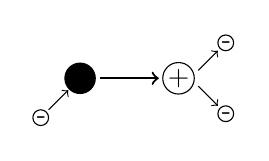
\begin{tikzpicture}
		    \node at (-0.49,-0.5) {-};
		    \node at (1.86,0.45) {-};
		    \node at (1.86,-0.45) {-};
		    \node at (1.25,0.0) {+};
		    \draw (-0.5,-0.5) circle (0.1);
		    \draw[->] (-0.4, -0.4) -- ( -0.15 , -0.15);
		    \fill     (0 , 0) circle (0.2);
		    \draw [->, thick] (0.25, 0.0) -- (1.0,0.0);
		    \draw (1.25, 0.0) circle (0.2);
		    \draw[->] (1.5, 0.1) -- (1.75, 0.35);
		    \draw[->] (1.5, -0.1) -- (1.75, -0.35);
		    \draw (1.85, 0.45) circle (0.1);
		    \draw (1.85, -0.45) circle (0.1);
	    \end{tikzpicture}
      }
	    \caption{}
    \end{subfigure}
    \begin{subfigure}{0.49\textwidth}
	    \centering
        \resizebox{0.8\textwidth}{!}{
 	      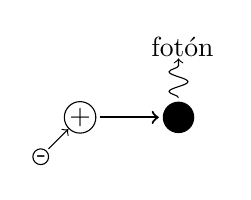
\begin{tikzpicture}
		      \node at (-0.49,-0.5) {-};
		      \node at (0.0,0.0) {+};
		      \draw (-0.5,-0.5) circle (0.1);
		      \draw[->] (-0.4, -0.4) -- ( -0.15 , -0.15);
		      \draw (0 , 0) circle (0.2);
		      \draw [->, thick] (0.25, 0.0) -- (1.0,0.0);
		      \fill (1.25, 0.0) circle (0.2);
		      \draw[->, decorate, decoration={snake, amplitude=1.2mm, segment length=2.5mm}] (1.25,0.25) -- (1.25,0.75);
		      \node at (1.30,0.90) {fot\'on};
      \end{tikzpicture}
      }
	    \caption{}
    \end{subfigure}
    \caption{Diagrama de colisiones en un plasma (a) ionizaci\'on/recombinaci\'on por colisi\'on entre especies. (b) recombinaci\'on/ionizaci\'on por procesos radiativos. N\'otese que se las flechas son invertibles para obtener los procesos inversos }
  \end{figure}
